\documentclass{article}
\usepackage{graphicx}
\usepackage{listings}
\usepackage{xcolor}
\usepackage{amsmath}
\usepackage[a4paper, margin=1in]{geometry}
\setlength{\parindent}{0pt}

\title{Week6 Lab2 Report}
\author{111062117, Hsiang-Sheng Huang}

\begin{document}

\maketitle

\section*{Matrix Multiplication Profiler}

\subsection*{Observations}

Execute the three files directly to measure the execution time.

\begin{figure}[htbp]
    \centering
    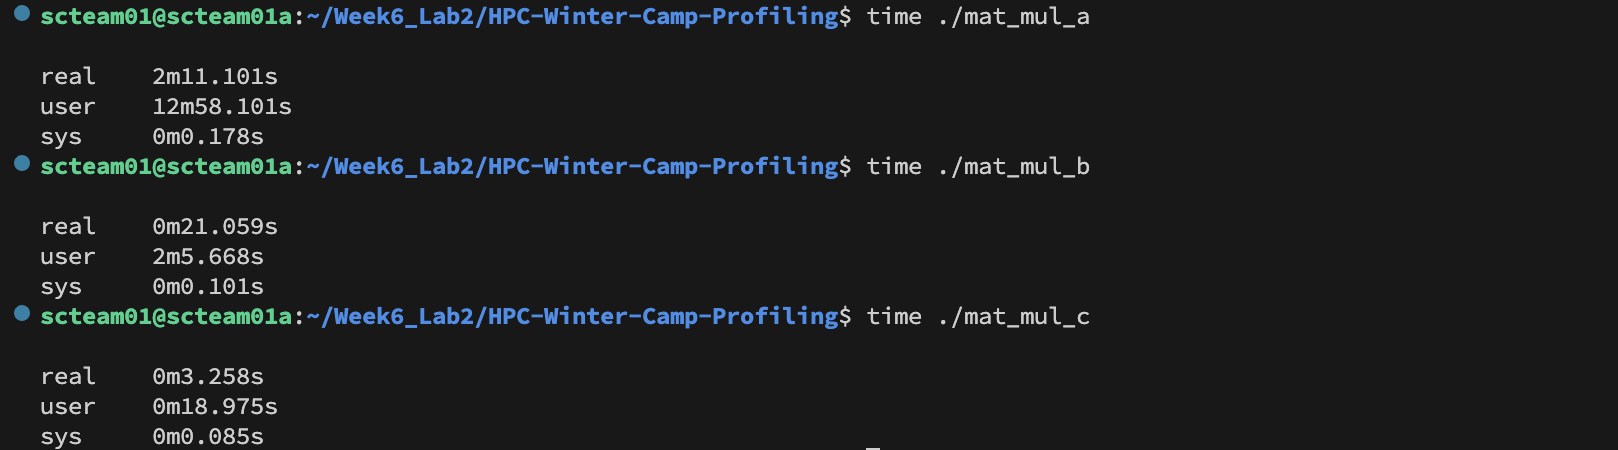
\includegraphics[width=1\textwidth]{./img/q1-1.png}
\end{figure}

\subsection*{Running APS}

Run APS to observe the elapsed time and memory usage.

\begin{figure}[htbp]
    \centering
    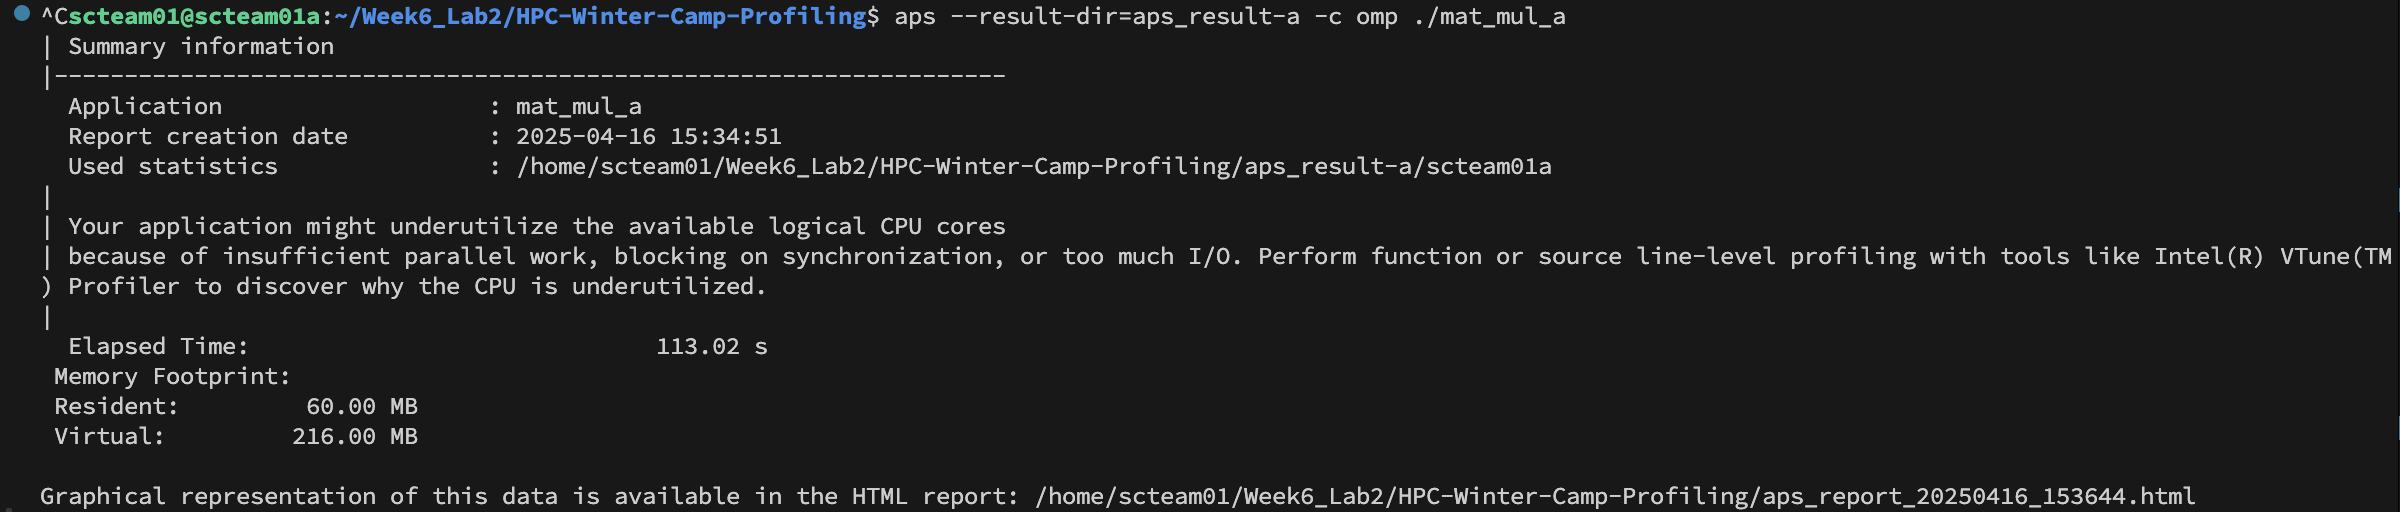
\includegraphics[width=1\textwidth]{./img/q1-2.png}
\end{figure}

\begin{figure}[htbp]
    \centering
    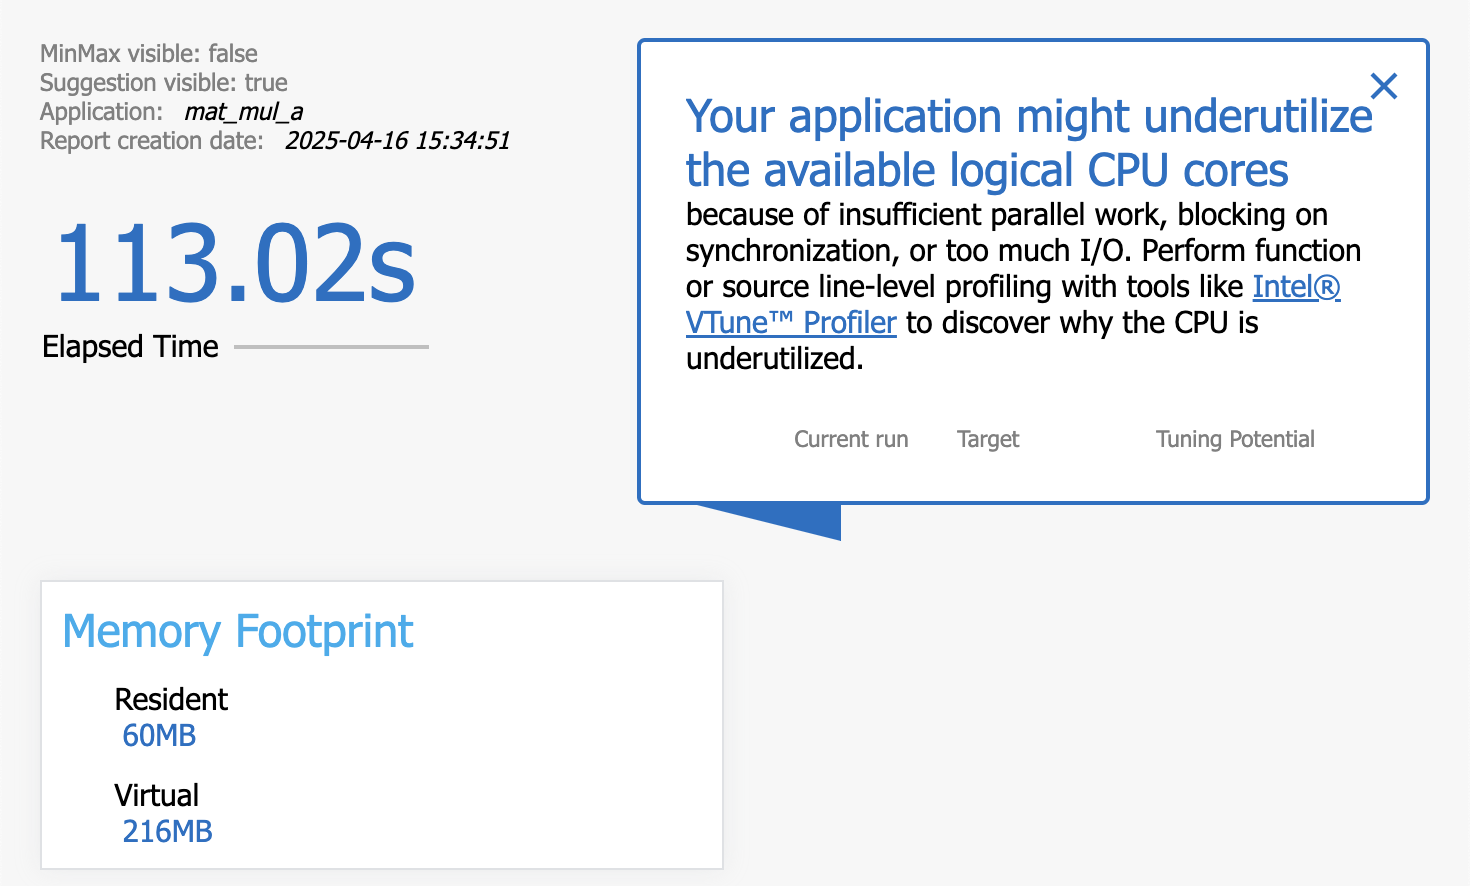
\includegraphics[width=1\textwidth]{./img/q1-3.png}
\end{figure}

\begin{figure}[htbp]
    \centering
    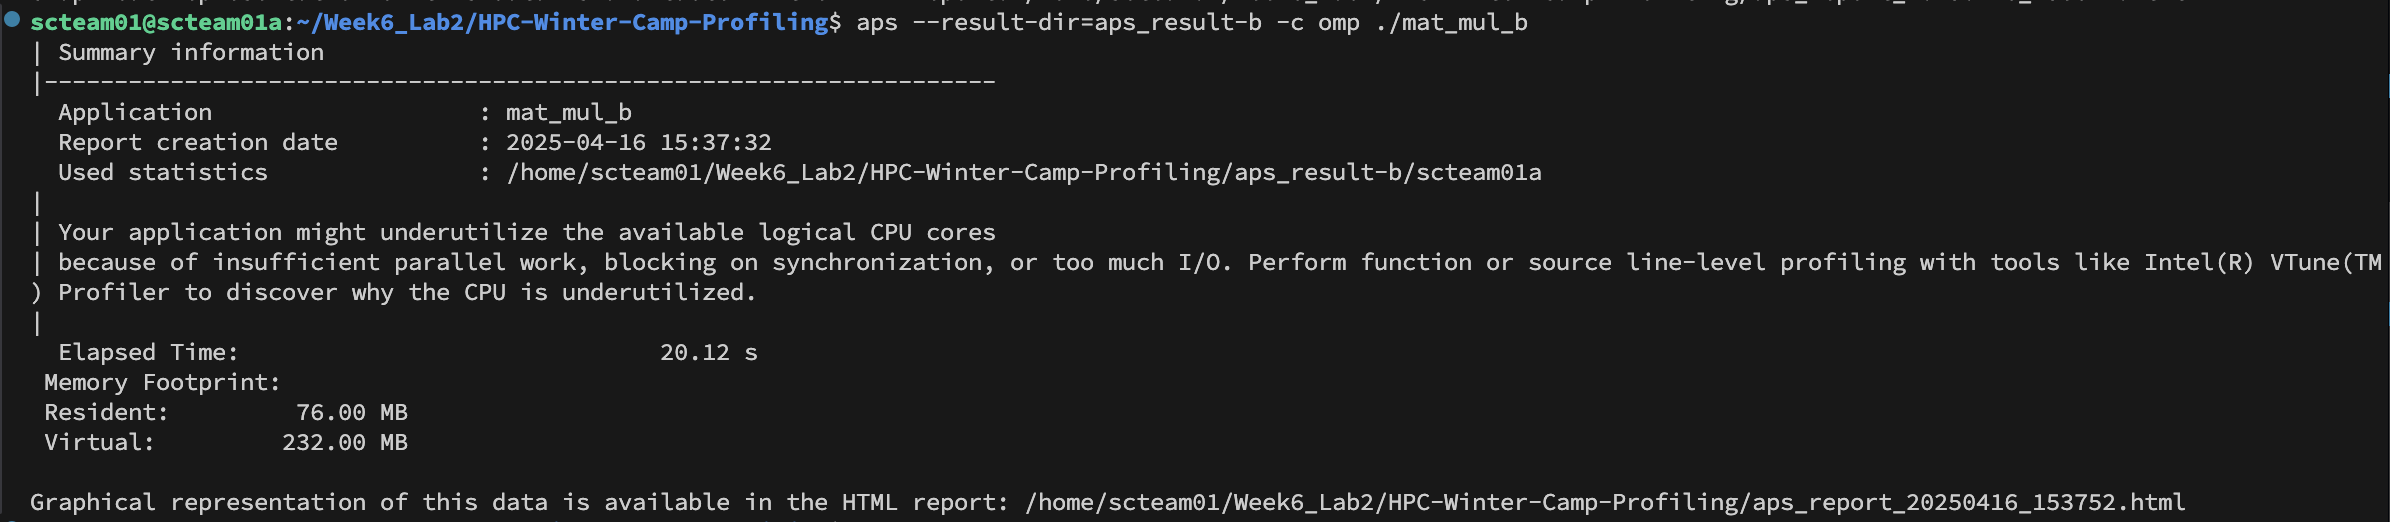
\includegraphics[width=1\textwidth]{./img/q1-4.png}
\end{figure}

\begin{figure}[htbp]
    \centering
    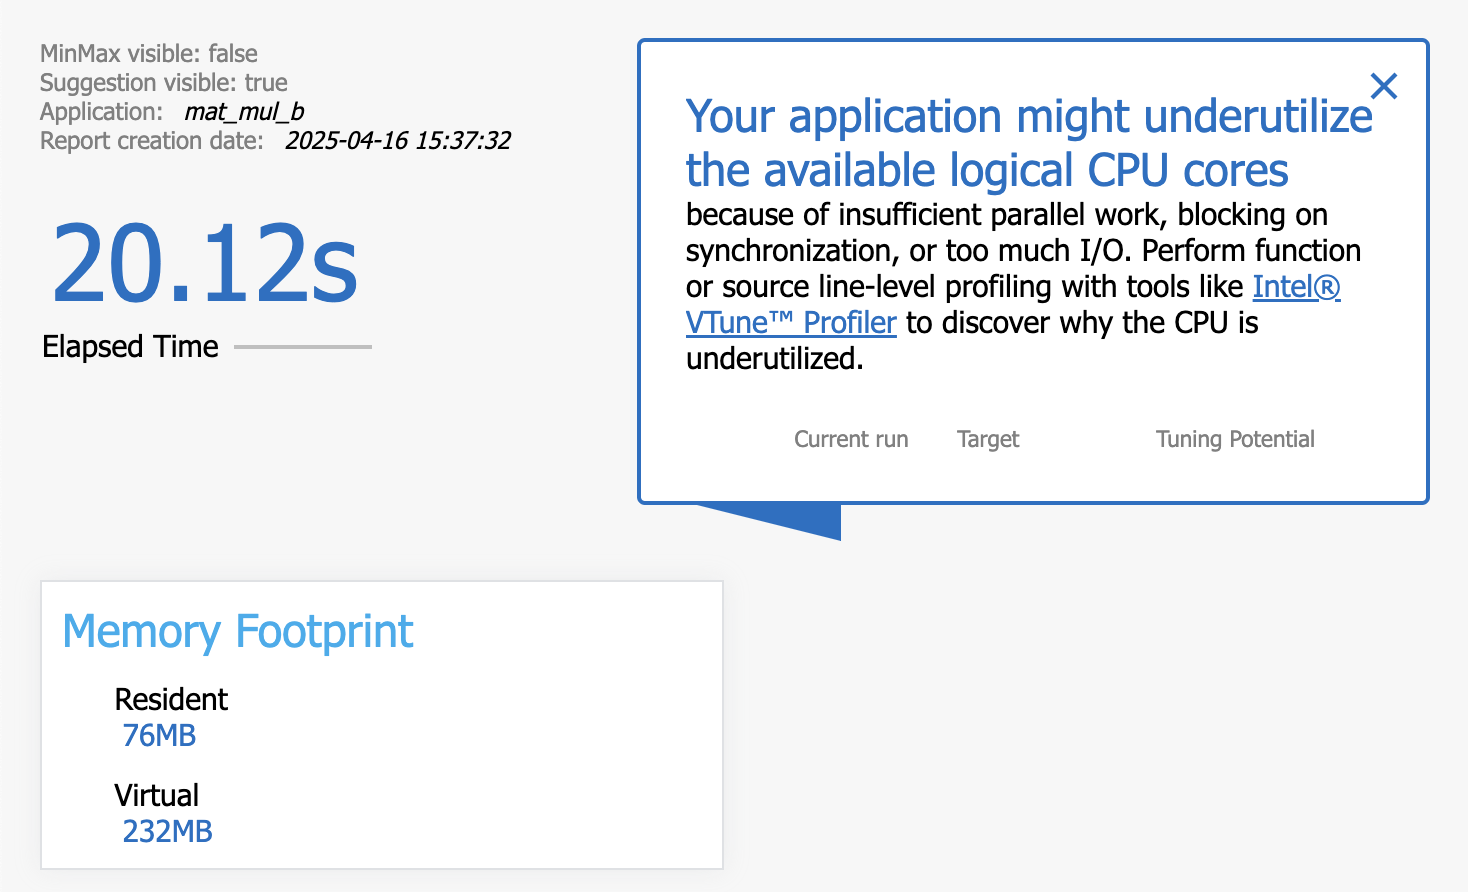
\includegraphics[width=1\textwidth]{./img/q1-5.png}
\end{figure}

\begin{figure}[htbp]
    \centering
    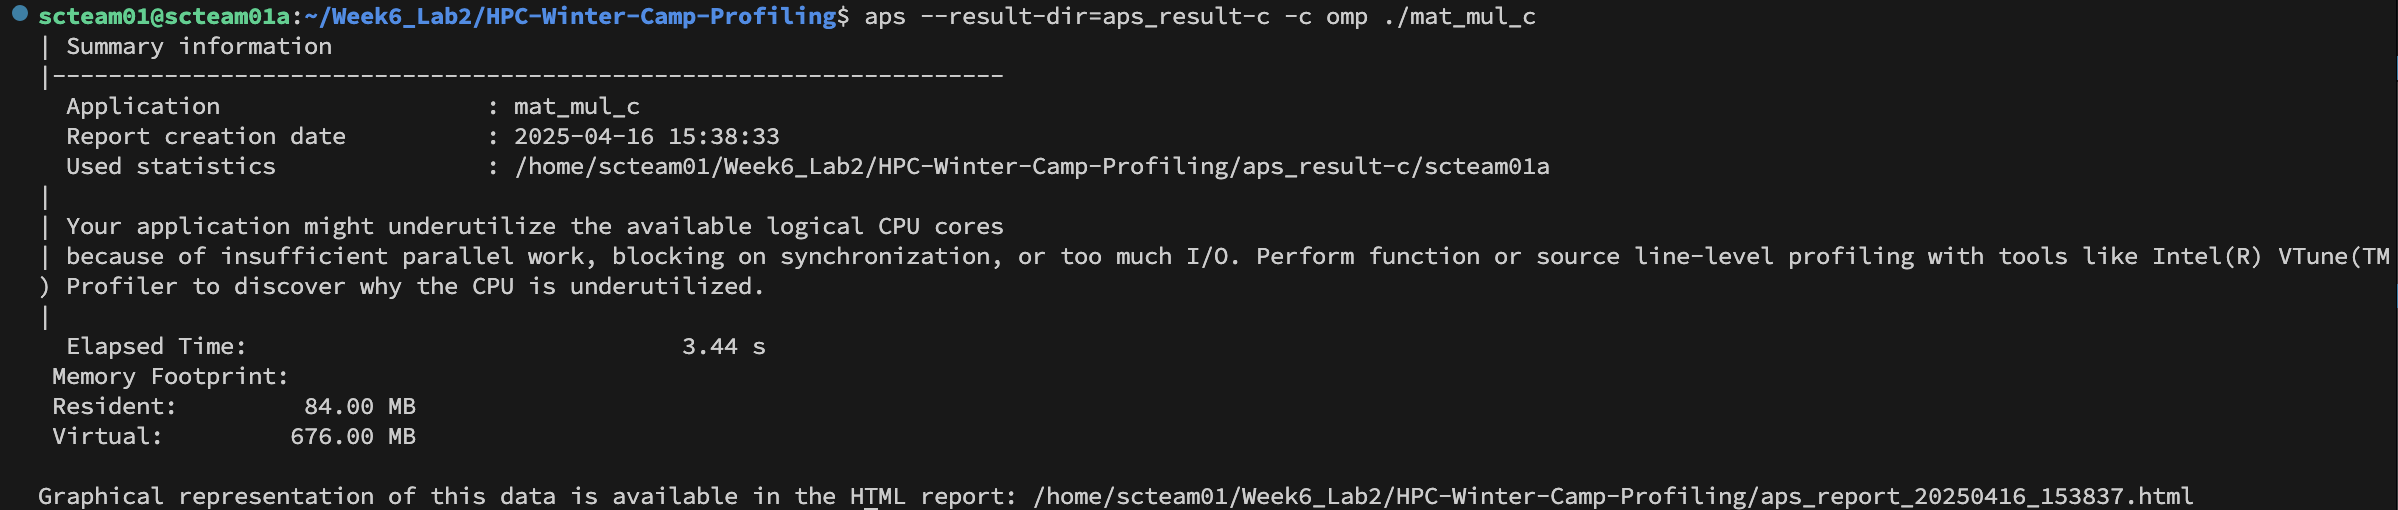
\includegraphics[width=1\textwidth]{./img/q1-6.png}
\end{figure}

\begin{figure}[htbp]
    \centering
    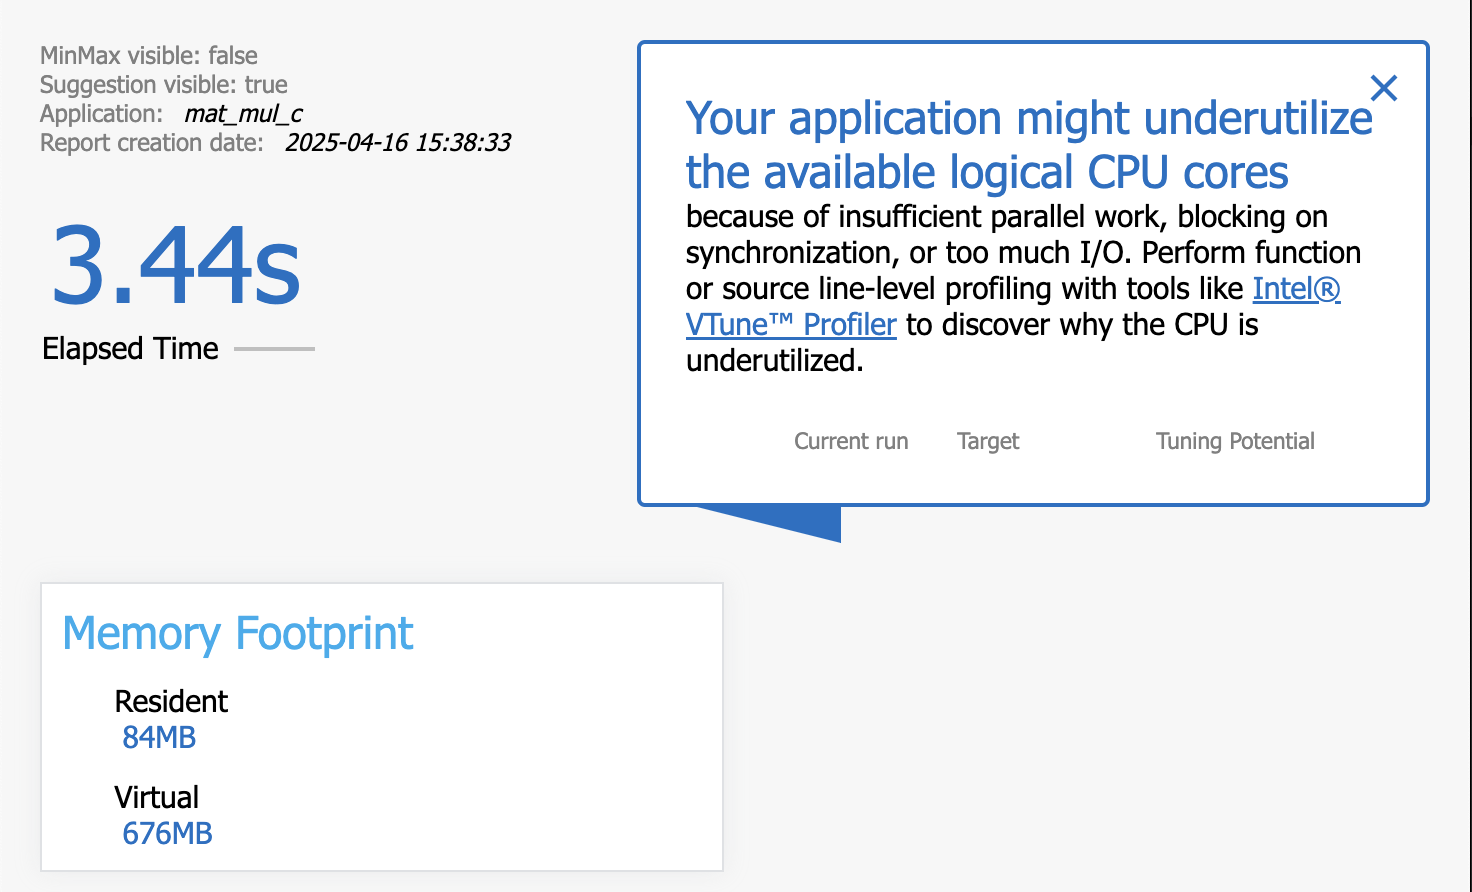
\includegraphics[width=1\textwidth]{./img/q1-7.png}
\end{figure}

\clearpage

\subsection*{Vtune}

Run VTune Hotspots to identify the most time-consuming functions or sections.

\begin{figure}[htbp]
    \centering
    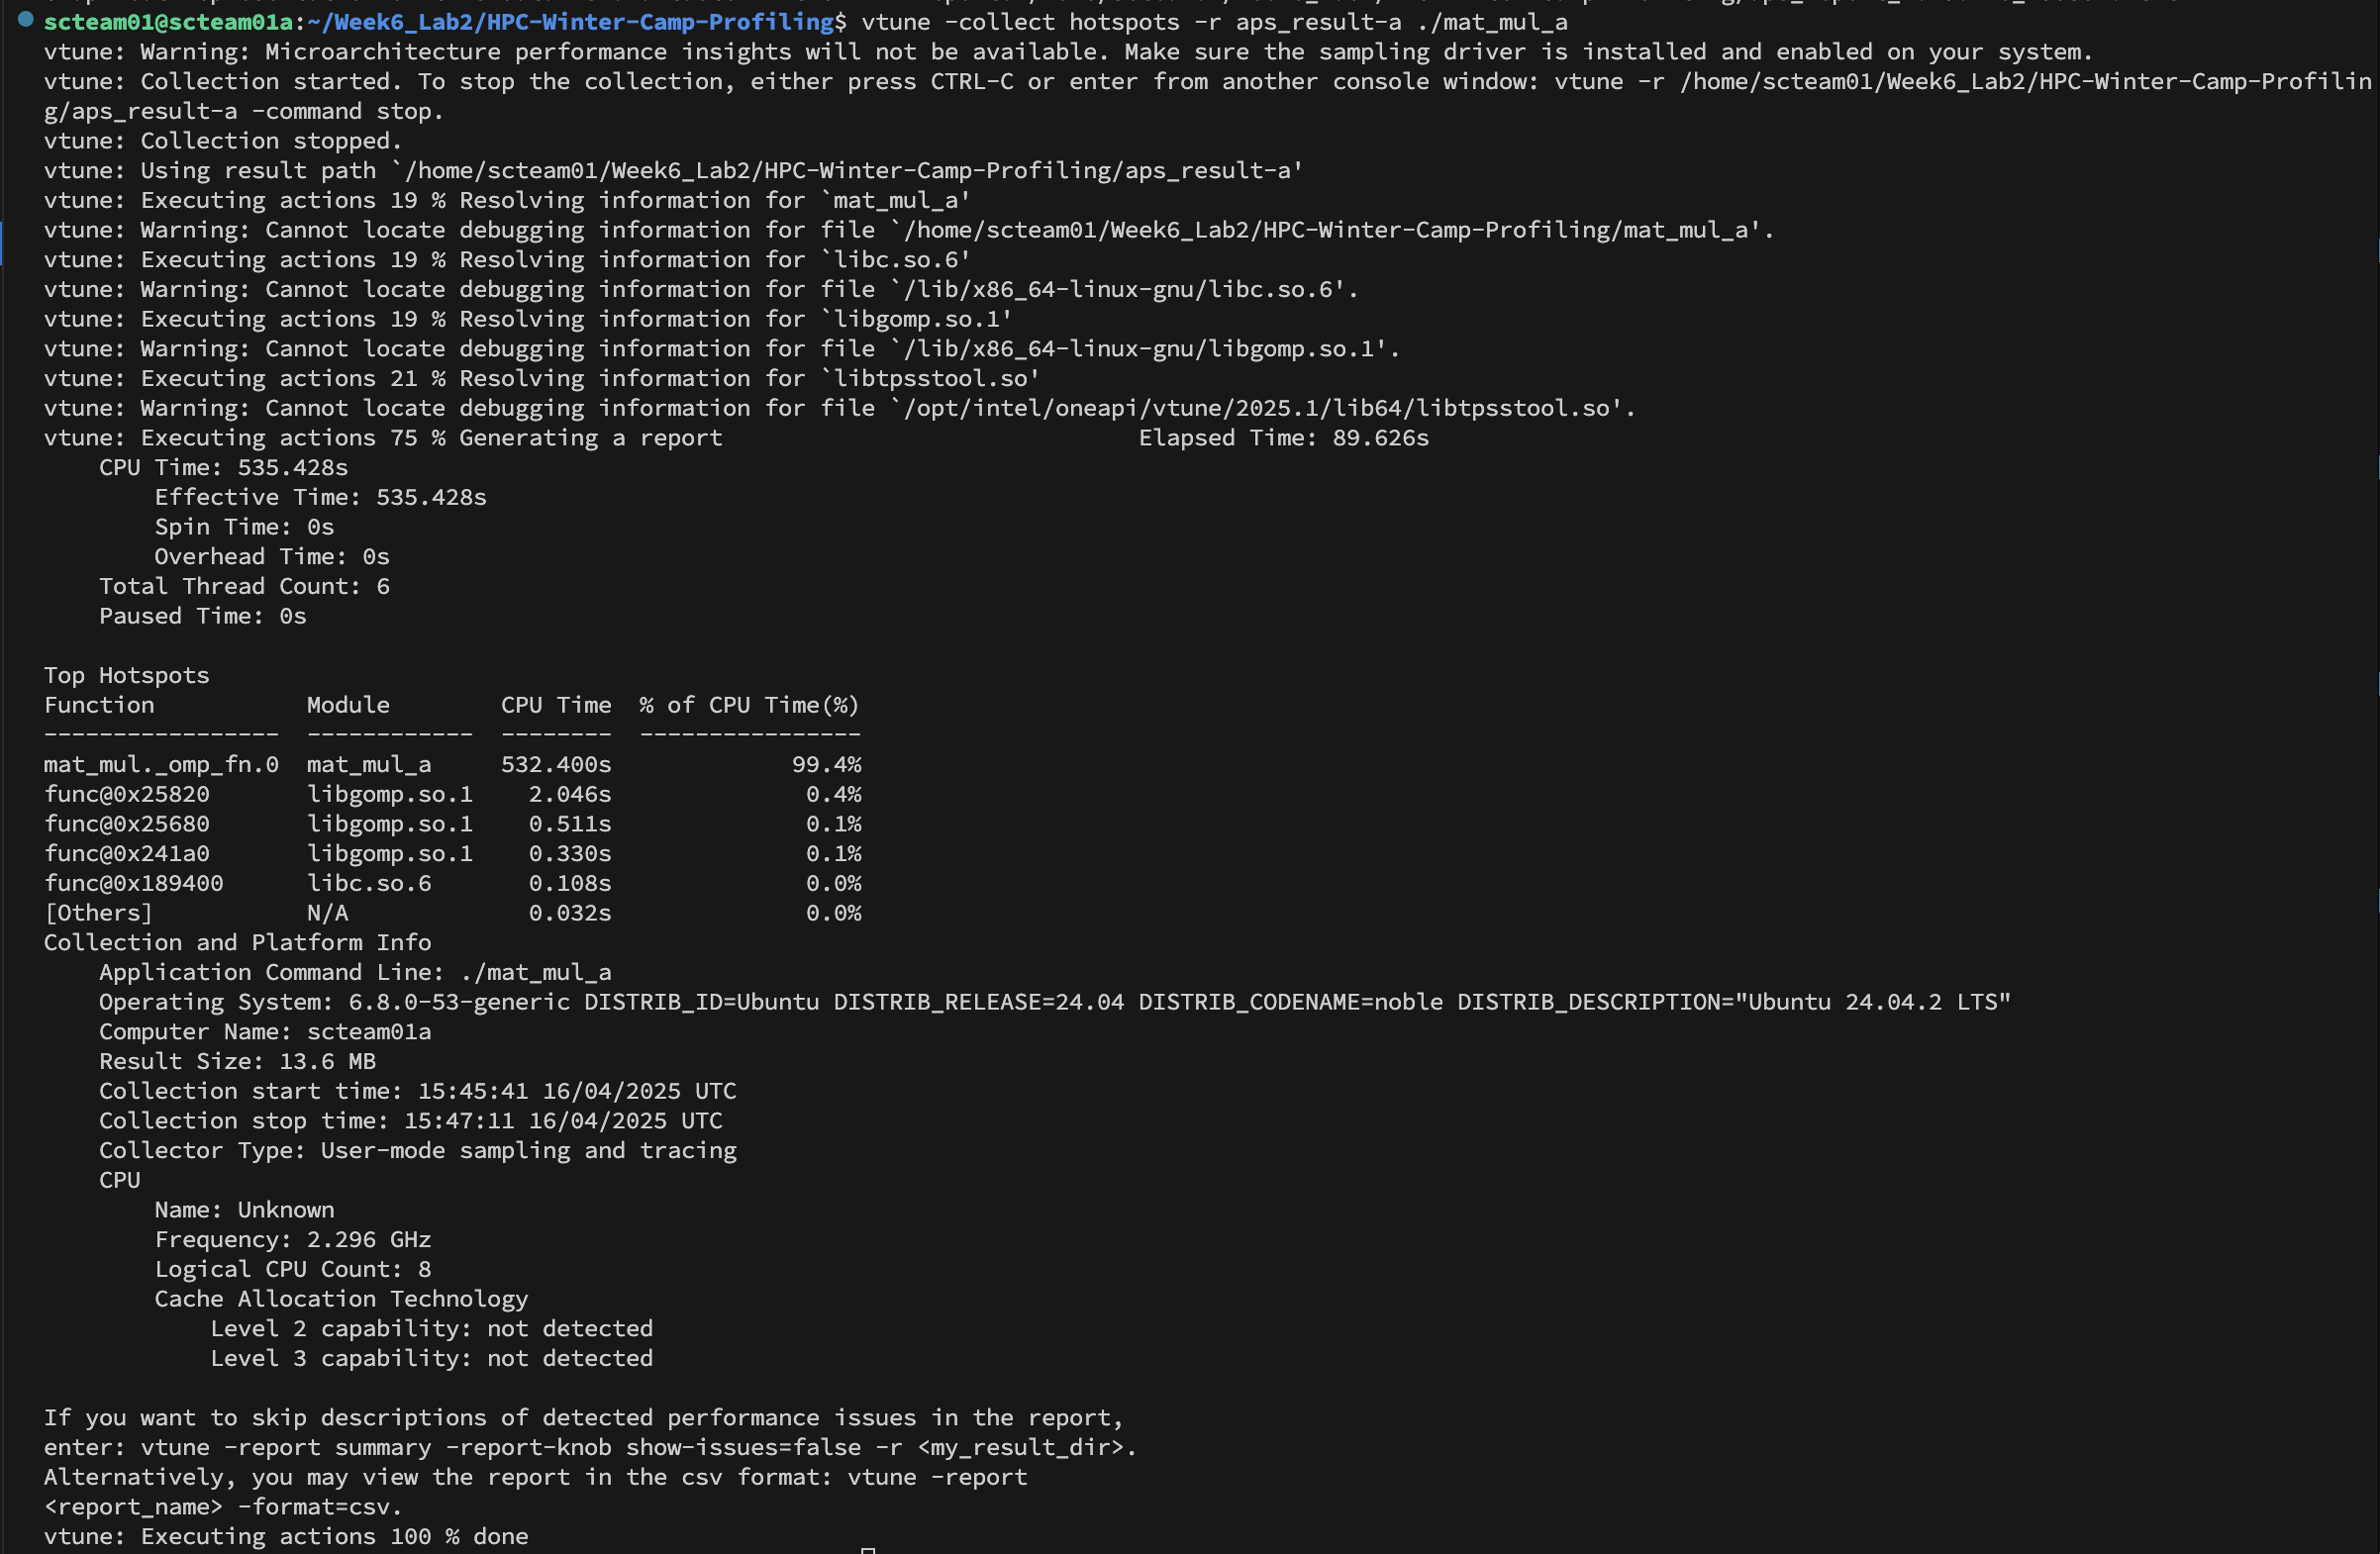
\includegraphics[width=1\textwidth]{./img/q1-8.png}
\end{figure}

\section*{MPI}

\subsection*{Screenshot of Successful execution}

I wrote a shell script to test cases with $n = (512, 1024, 2048)$. The shell script is as follows:

\begin{lstlisting}[language=bash, basicstyle=\ttfamily\small, numbers=left, numberstyle=\tiny\color{gray}, stepnumber=1, frame=single, showstringspaces=false]
    #!/bin/bash

    # Clean and compile all necessary files
    make clean
    make
    
    # Matrix sizes to test
    Ns=(512 1024 2048)
    
    # MPI configuration
    NP=4      # number of processes
    NX=2      # number of blocks in x-direction
    NY=2      # number of blocks in y-direction
    
    # Run for each matrix size
    for N in "${Ns[@]}"
    do
        echo "========== Running for N = $N =========="
    
        echo "[1] Generating A.out and B.out"
        ./generator "$N"
    
        echo "[2] Running MPI matrix multiplication"
        START=$(date +%s.%N)
        mpirun -np $NP ./matrix-mpi "$N" "$NX" "$NY"
        END=$(date +%s.%N)
        RUNTIME=$(echo "$END - $START" | bc)
        echo "    Total execution time: $RUNTIME seconds"
    
        # Optionally, calculate FLOPS based on theoretical operations (2 * N^3)
        FLOPS=$(echo "scale=2; 2 * $N * $N * $N / $RUNTIME" | bc)
        GFLOPS=$(echo "scale=2; $FLOPS / 1e9" | bc)
        echo "    Calculated performance: $FLOPS FLOPS"
        echo "    Calculated performance: $GFLOPS GFLOPS"
    
        echo "[3] Comparing results using float-diff"
        if [ -f C.out ]; then
            ./float-diff C.out output.out
            STATUS=$?
            if [ $STATUS -eq 0 ]; then
                echo "    Output is correct (no significant difference)"
            else
                echo "    Output mismatch detected"
            fi
        else
            echo "    C.out not found, skipping comparison"
        fi
    
        echo ""
    done
\end{lstlisting}

And the result is as follows: 

\begin{figure}[htbp]
    \centering
    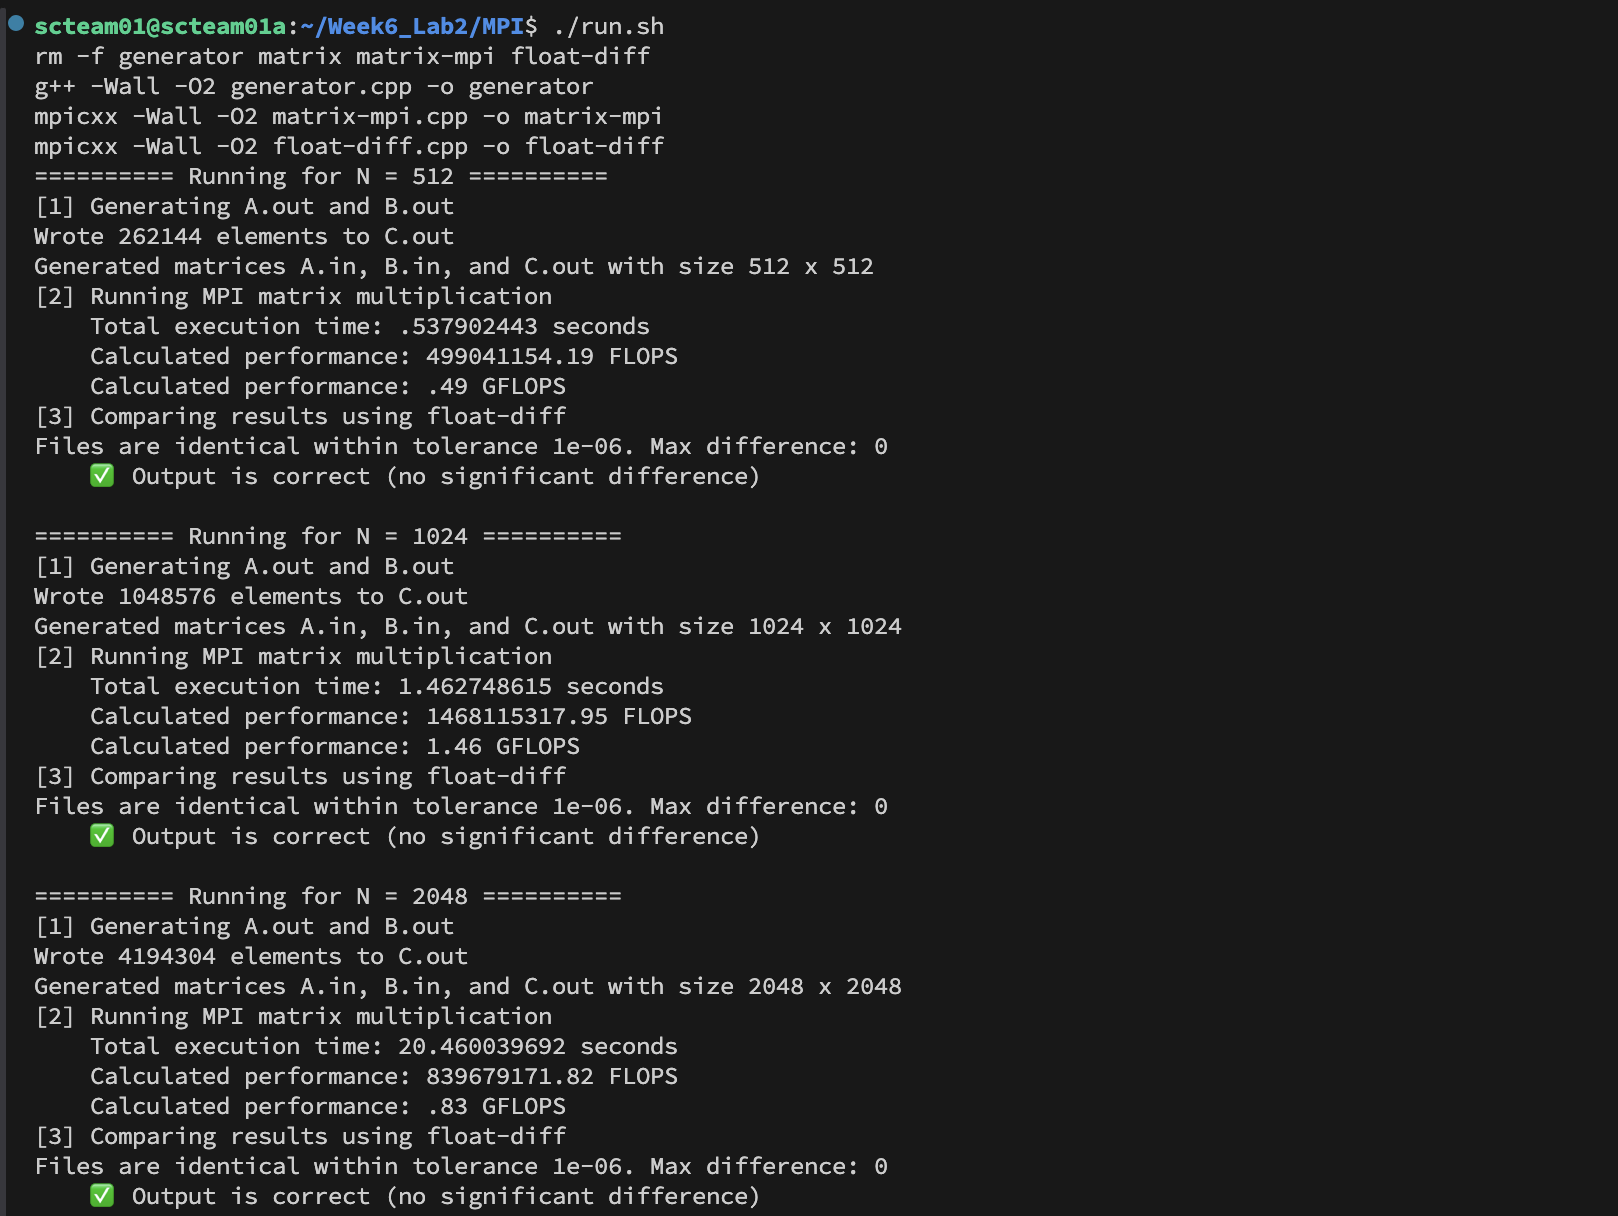
\includegraphics[width=1\textwidth]{./img/q2-1.png}
\end{figure}

\subsection*{Understanding / Modifying / Optimizing the code}

\subsubsection*{generator.cpp}
This file generates the input matrices A and B with random values for testing.

Key functionality:
\begin{itemize}
    \item Creates two matrices of size $N \times N$ with random float values
    \item Writes these matrices to A.out and B.out files
    \item Also computes the sequential matrix multiplication result and saves to C.out for verification
\end{itemize}

\subsubsection*{matrix-mpi.cpp}
This file implements the parallel matrix multiplication using MPI.

Key components:
\begin{itemize}
    \item MPI initialization and process configuration (rank, size)
    \item Data distribution: divides matrices into blocks according to NX and NY parameters
    \item Communication pattern between processes for exchanging matrix blocks
    \item Local computation of partial results
    \item Gathering final results to the root process
\end{itemize}

Optimization Strategies:

\begin{itemize}
    \item \textbf{Block-Cyclic Distribution}: Instead of simple block distribution, implementing a block-cyclic distribution could improve load balancing, especially for larger matrices.
    \item \textbf{Overlapping Communication and Computation}: Using non-blocking MPI operations (e.g., MPI\_Isend, MPI\_Irecv) to overlap communication with computation.
    \item \textbf{Hierarchical Parallelism}: Combining MPI with OpenMP for hybrid parallelism - using MPI across nodes and OpenMP threads within each node.
    \item \textbf{Algorithmic Improvements}: Implementing Cannon's algorithm or SUMMA (Scalable Universal Matrix Multiplication Algorithm) which are designed to minimize communication overhead.
    \item \textbf{Memory Optimization}: Using local memory efficiently through cache blocking techniques to improve spatial and temporal locality.
    \item \textbf{Communication Reduction}: Reorganizing the algorithm to minimize the total volume of data exchanged between processes.
\end{itemize}

\subsubsection*{float-diff.cpp}
This utility compares the output matrices to verify correctness.

Key functionality:
\begin{itemize}
    \item Reads two matrix files and compares their values
    \item Allows for small floating-point differences (epsilon tolerance)
    \item Returns success (0) if matrices match within tolerance
\end{itemize}

\subsection*{Profile results}

The result is as follows:

\begin{figure}[htbp]
    \centering
    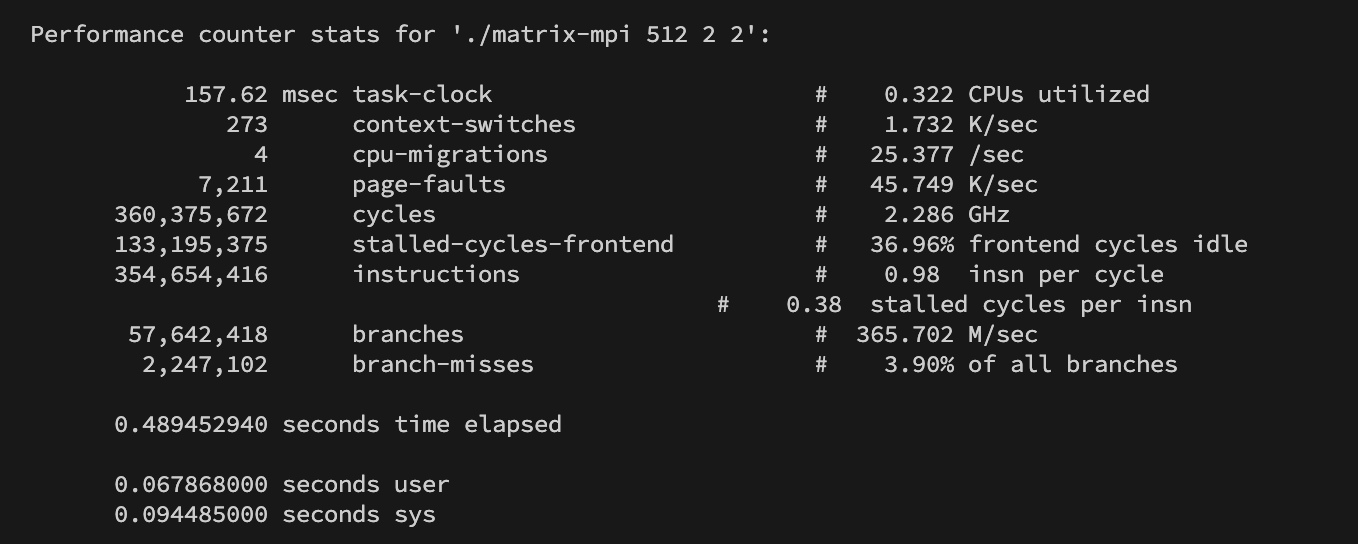
\includegraphics[width=1\textwidth]{./img/q2-2.png}
\end{figure}

The profiling results provide valuable insights into the performance characteristics of our MPI implementation. The key observations are:

\begin{itemize}
    \item \textbf{CPU Utilization}: At 0.322 CPUs utilized, our implementation shows relatively low CPU efficiency, suggesting potential for better parallelism or resource usage.
    
    \item \textbf{Cache and Memory Behavior}: The high number of page faults (7,211) indicates frequent memory access outside the working set, which could be a performance bottleneck.
    
    \item \textbf{Pipeline Efficiency}: With 36.96\% frontend cycles idle and a instructions per cycle (IPC) ratio of 0.98, the processor is spending significant time waiting, likely due to memory access latency.
    
    \item \textbf{Branch Prediction}: The 3.90\% branch misprediction rate is reasonable but could be improved for better instruction flow.
    
    \item \textbf{Overall Performance}: The total execution time of 0.489 seconds for a $512 \times 512$ matrix multiplication demonstrates the effectiveness of parallelization, but the metrics suggest room for optimization, particularly in memory access patterns and CPU utilization.
\end{itemize}

These metrics suggest that optimizing memory locality and reducing communication overhead would likely yield significant performance improvements for larger matrix sizes.

\subsection*{Computational Performance (GFLOPS)}

\subsubsection*{Theoretical FLOPS Calculation}
For matrix multiplication of two $N \times N$ matrices, the operation count can be derived as follows:

\begin{itemize}
    \item For each element in the result matrix, we compute the dot product of a row from matrix A and a column from matrix B
    \item Each dot product requires $N$ multiplications and $N-1$ additions
    \item Therefore, each element requires approximately $2N$ floating-point operations (for large $N$)
    \item With $N^2$ elements in the result matrix, the total operation count is approximately $2N^3$
\end{itemize}

This is why we use $2N^3$ floating-point operations in our GFLOPS calculation:
\begin{align*}
    \text{GFLOPS} &= \frac{\text{Total Operations}}{\text{Execution Time (seconds)}} \\
    &= \frac{2N^3 \text{ operations}}{\text{Execution Time (seconds)}} \\
    &= \frac{2N^3}{10^9} \cdot \text{GFLOPS}
\end{align*}

\begin{table}[htbp]
    \centering
    \begin{tabular}{|c|c|c|c|}
        \hline
        \textbf{Matrix Size (N)} & \textbf{Execution Time (s)} & \textbf{GFLOPS} \\
        \hline
        512 & 0.5379 & 0.49 \\
        \hline
        1024 & 1.4627 & 1.46 \\
        \hline
        2048 & 20.4600 & 0.83 \\
        \hline
    \end{tabular}
    \caption{Computational performance for different matrix sizes}
\end{table}

\end{document}
